\documentclass[12pt, a4paper]{article}

\usepackage{array}
\usepackage[portuguese]{babel}
\usepackage{float}
\usepackage[a4paper, margin=2cm]{geometry}
\usepackage{graphicx}
\usepackage{hyperref}
\usepackage{pdfpages}
\usepackage{setspace}

\title{\textbf{Interface Pessoa-Máquina \\ \large Trabalho Prático -- Fase II}}
\date{4 de maio de 2025}
\author{Grupo 12 \\ \\
    \url{https://www.figma.com/design/Ps4VLCPz66bKq5p2ypzrDR/Projeto-IPM} \\ \\
    \url{https://github.com/UMinho-ENGINF-IPM/trabalho-pr-tico-gp25_12}}

\begin{document}

\begin{center}
    
\includegraphics[width=0.25\textwidth]{res/cover/school-of-engineering.eps}
\end{center}

{\let\newpage\relax\maketitle}
\maketitle
\thispagestyle{empty}

\chardef\_=`_
\onehalfspacing
\setlength{\parskip}{\baselineskip}
\setlength{\intextsep}{2\baselineskip}
\setlength\belowcaptionskip{-\baselineskip}
\setlength{\parindent}{0pt}
\def\arraystretch{1.5}

\begin{center}
    \begin{tabular}{>{\centering}p{0.25\textwidth}
                    >{\centering}p{0.25\textwidth}
                    >{\centering\arraybackslash}p{0.25\textwidth}}
        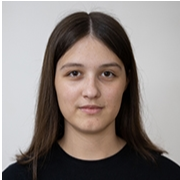
\includegraphics[width=3.5cm]{res/cover/A104437.png} &
        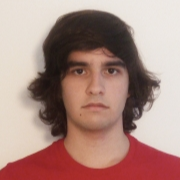
\includegraphics[width=3.5cm]{res/cover/A104348.png} &
        
\includegraphics[width=3.5cm]{res/cover/A104263.png}  \\

        Ana Oliveira & Humberto Gomes & Inês Marques \\
        A104437      & A104348        & A104263
    \end{tabular}

    \begin{tabular}{>{\centering}p{0.25\textwidth}
                    >{\centering\arraybackslash}p{0.25\textwidth}}
        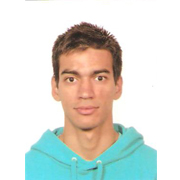
\includegraphics[width=3.5cm]{res/cover/A76350.jpg} &
        
\includegraphics[width=3.5cm]{res/cover/A104179.png} \\

        Rafael Vilas Boas & Sara Lopes \\
        A76350            & A104179
    \end{tabular}
\end{center}

\begin{abstract}
    \noindent
    No âmbito da segunda fase deste trabalho prático, foi implementada, com base em modelação
    prévia, uma interface de utilizador de um sistema para a gestão de horários de um curso
    universitário, utilizado tanto pelos alunos como pelo diretor de curso. Neste documento,
    apresenta-se a interface implementada em Vue \cite{vue} (e outras tecnologias) e o seu processo
    de implementação, bem como algumas correções feitas ao modelo da interface. Por falta de tempo,
    não foi possível fazer testes da aplicação com utilizadores reais, não sendo possível fazer uma
    reflexão muito aprofundada sobre a qualidade do produto final. No entanto, consideramos que a
    aplicação desenvolvida cumpriu os requisitos pedidos.
\end{abstract}

\section{Objetivos}

O objetivo do trabalho prático proposto na Unidade Curricular de Interface Pessoa-Máquina é a
modelação e o desenvolvimento de uma aplicação Web para para a gestão de horários de um curso
universitário, utilizado tanto pelos alunos como pelo diretor de curso. Em particular, deseja-se que
a aplicação permita aos alunos consultar o seu horário e fazer pedidos de troca de turno ao diretor
de curso, e que o diretor de curso possa manualmente colocar alunos em turnos (para resolver
limitações do algoritmo de colocação e aceder a pedidos de alunos) e aceder a pedidos de professores
para mudança de turnos para salas maiores. Para mais detalhes, o enunciado do trabalho prático pode
ser consultado nos anexos deste relatório. Idealmente, a aplicação deve ajudar o utilizador a não
cometer erros, como colocar alunos em turnos que originem sobreposições de horário.

Na primeira fase deste trabalho, fez-se a modelação da aplicação em Figma \cite{figma}, e nesta
fase, procurou-se implementar a interface modelada em Vue \cite{vue}. Também se realizaram algumas
alterações ao modelo, a corrigir alguns aspetos que se acharam relevantes.

\section{Alterações ao Modelo da Interface}

Na fase anterior deste trabalho prático, construiu-se, em Figma \cite{figma}, um modelo da interface
a implementar. Apesar de uma boa avaliação nesta fase, a docência da UC de Interface Pessoa-Máquina
reparou em alguns aspetos que podiam ser melhorados. Nesta secção, apresentam-se as mudanças que
foram feitas ao modelo da interface devido tanto aos comentários dos docentes como a outros aspetos
que o grupo de trabalho se apercebeu que podiam ser melhorados.

Em primeiro lugar, a página ``Iniciar Sessão'' não é ideal para a prevenção de erros: é possível que
o utilizador submeta parcialmente as suas credenciais (apenas o seu endereço eletrónico ou apenas a
sua palavra-passe), e o sistema reagirá com um erro. Para prevenir este erro, deve ser impossível
que um utilizador submeta as suas credenciais até as escrever todas. Logo, na nova versão do modelo
da interface, o botão de submissão de credenciais encontra-se desativado até o utilizador escrever
tanto o seu endereço eletrónico como a sua palavra-passe, como mostra a figura abaixo:

\begin{figure}[H]
    \centering
    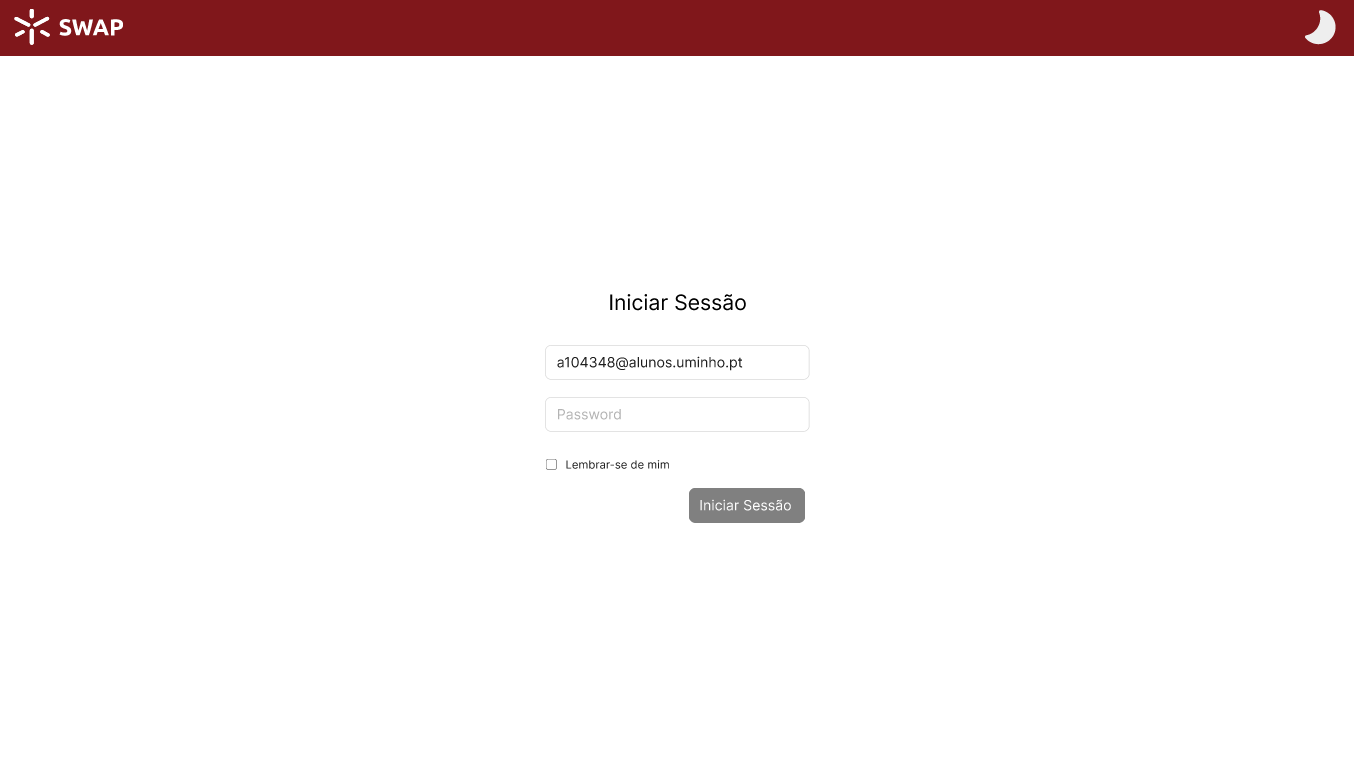
\includegraphics[width=0.8\textwidth]{res/prototype/iniciar-sessao-botao-desativado-email.png}
    \caption{Captura de ecrã do protótipo da página ``Iniciar Sessão'' com botão desativado.}
    \label{iniciar-sessao-botao-desativado-email}
\end{figure}


É importante que o utilizador saiba por que este botão se encontra desativado, pelo que, tal como
foi feito em outros botões na interface, uma \emph{tooltip} foi utilizada para justificar por que
não é possível interagir com o botão:

\begin{figure}[H]
    \centering
    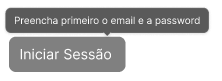
\includegraphics[width=0.3\textwidth]{res/prototype/inicar-sessao-tooltip-botao-desativado.png}
    \caption{\emph{Tooltip} sobre o botao de início de sessão desativado.}
    \label{inicar-sessao-tooltip-botao-desativado}
\end{figure}

Ademais, na página ``Resolver Problemas'', o título da página foi removido, e substituído por uma
barra de pesquisa. Em primeiro lugar, o título da página não era necessário, visto que o utilizador
já sabe em que página se encontra olhando para a hiperligação realçada na barra de navegação.
Depois, o espaço que se ganha na barra lateral com a remoção deste título pode ser usado uma barra
de pesquisa, um elemento muito útil para procurar alunos em grandes listas de problemas (o cenário 1
aponta para 45 alunos sem turnos atribuídos).

\begin{figure}[H]
    \centering
    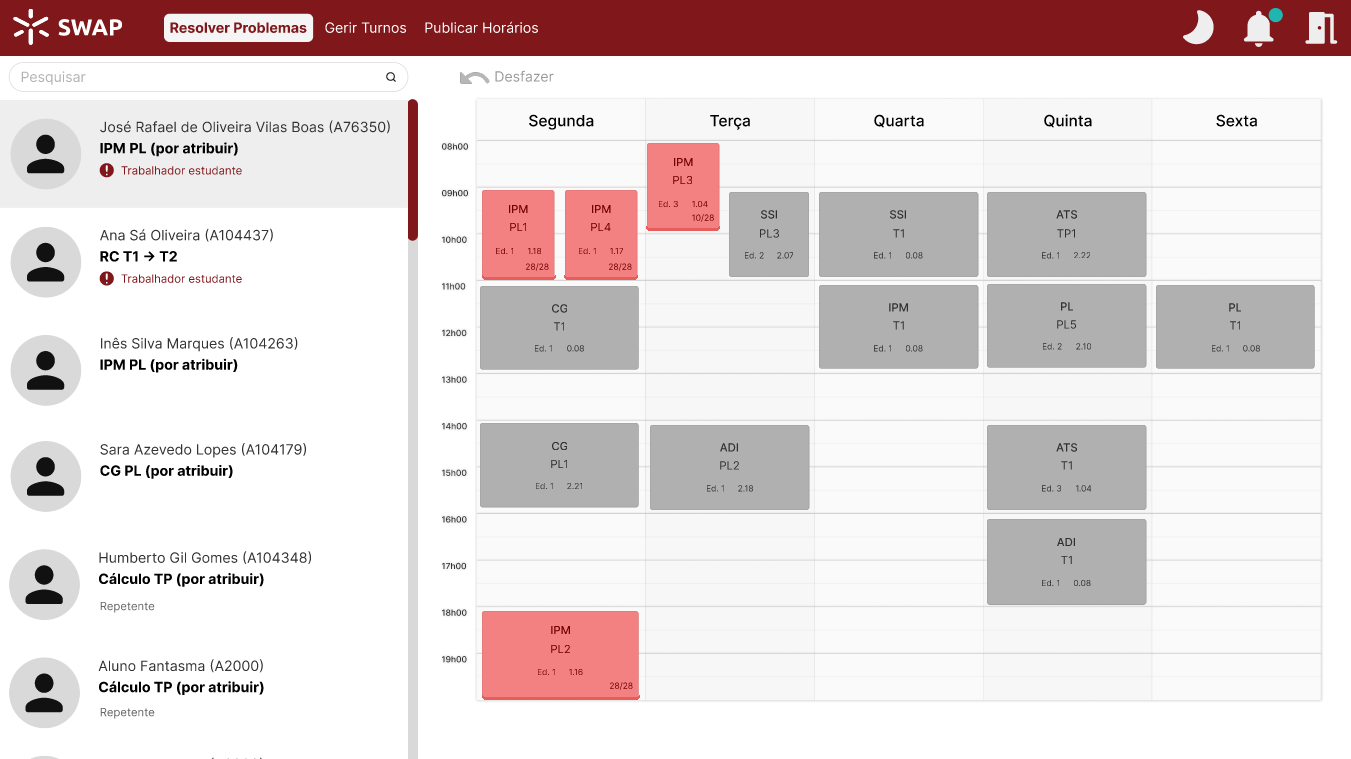
\includegraphics[width=0.8\textwidth]{res/prototype/resolver-problemas-revisto.png}
    \caption{Captura de ecrã do protótipo da página ``Resolver Problemas''.}
    \label{resolver-problemas-revisto}
\end{figure}

De seguida, uma sugestão da docência de Interface Pessoa-Máquina foi a eliminação da página
``Publicar Horários'', sendo estes atualizados sempre que o diretor de curso faz uma alteração. No
entanto, não consideramos esta solução viável, visto que o diretor de curso pode desejar colocar os
horários dos alunos em estados intermédios sem que estes os vejam. Por exemplo, pode desejar remover
vários alunos dos seus turnos, para os adicionar a outros turnos da mesma UC, assim, por exemplo,
abrindo vagas em turnos mais procurados. No entanto, reparou-se que é importante realçar quando as
mudanças feitas pelo diretor de curso ainda não são públicas. Por este motivo, tal como foi feito
para o ícone de notificações, quando há alterações por publicar, um pequeno círculo é adicionado ao
canto superior direito da hiperligação para a página ``Publicar Horário'', como mostra a figura
abaixo:

\begin{figure}[H]
    \centering
    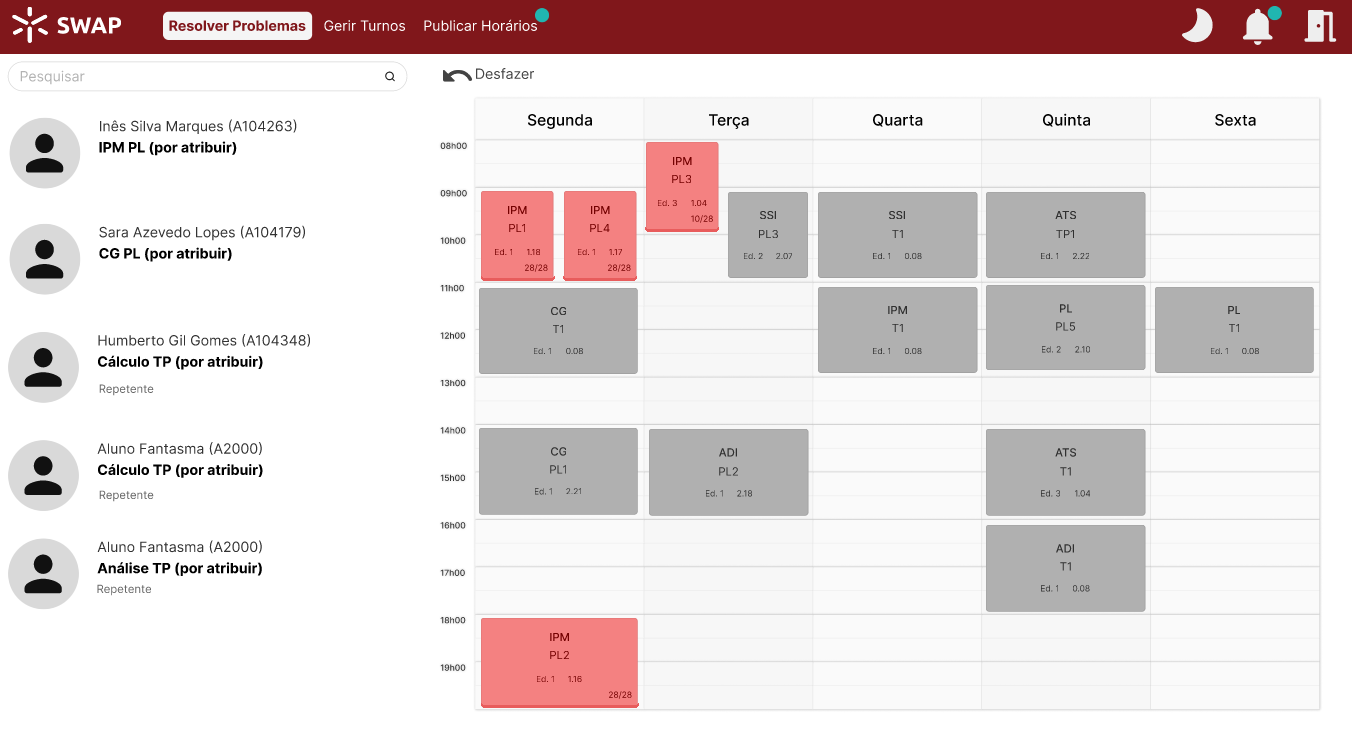
\includegraphics[width=0.8\textwidth]{res/prototype/mudancas-feitas-publicar-horario.png}
    \caption{Captura de ecrã do protótipo da página ``Resolver Problemas'' com mudanças feitas.}
    \label{mudancas-feitas-publicar-horario}
\end{figure}

No entanto, partindo da solução de não ser necessário publicar os horários, fez-se não ser
necessário, na página ``Gerir Turno'', guardar as alterações feitas a um turno: estas são guardadas
à medida que o utilizador as faz. Logo, o botão ``Guardar'' foi substituído por um botão ``Voltar''.
Na mesma página, desfazer uma alteração deixou de ser feito através de uma \emph{toast} que aparecia
sempre que uma alteração era feita, e sim por um botão ``Desfazer'', de forma consistente com a
página ``Resolver Problemas'':

\begin{figure}[H]
    \centering
    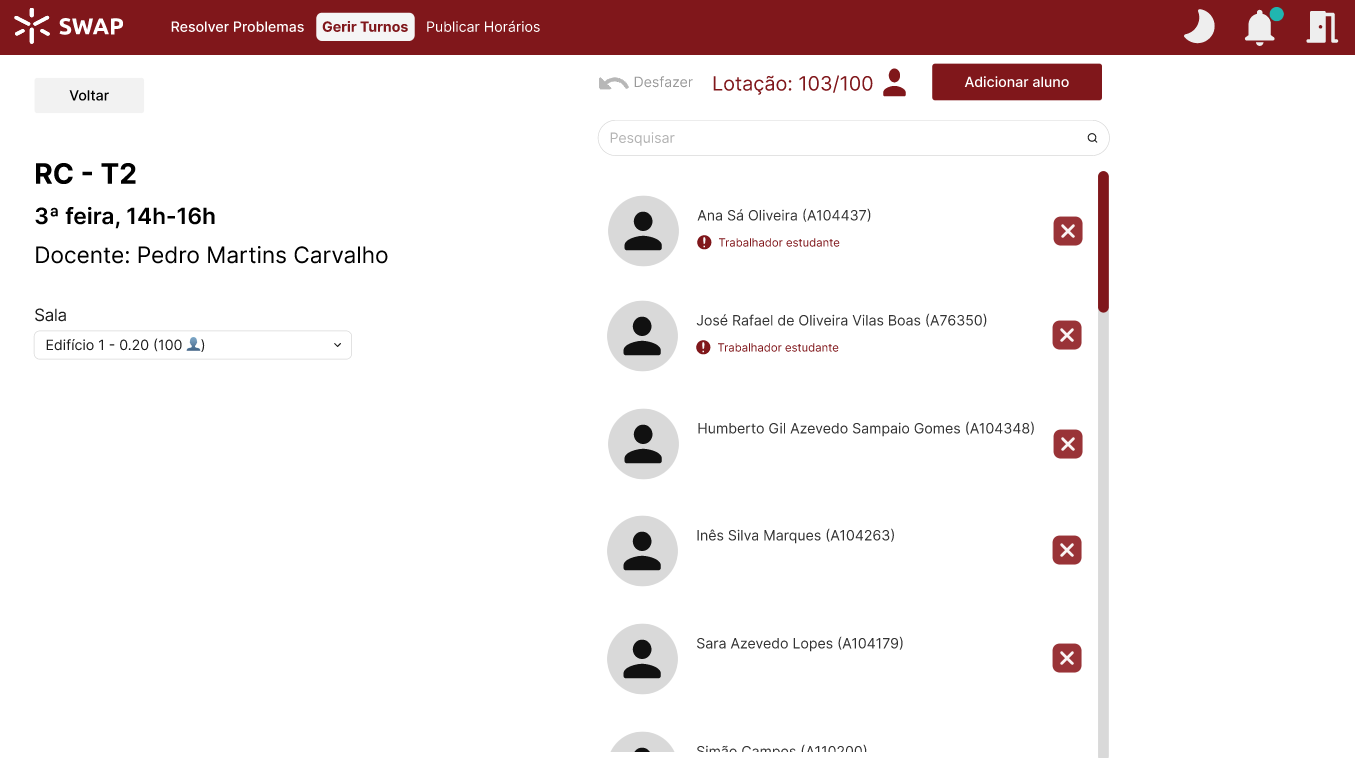
\includegraphics[width=0.8\textwidth]{res/prototype/gerir-turnos-revisto.png}
    \caption{Captura de ecrã do protótipo da página ``Gerir Turnos''.}
    \label{gerir-turnos-revisto}
\end{figure}

Na página ``Notificações'', o botão de alterar entre todas as notificações e as não lidas
foi removido, visto que as mesmas já se encontram separadas por este critério e ordenadas
cronológicamente.

{\color{red} TODO - figura}

Por último, também se seguiu a sugestão da equipa docente de mostrar o estado dos pedidos nas
páginas ``Histórico de Pedidos'' e ``Notificações do Diretor de Curso''. Abaixo, apresenta-se, como
exemplo, o modelo da página ``Histórico de Pedidos''. Apesar do uso de linguagem iconográfica, tal
como no resto da aplicação, os ícones apresentados têm todos \emph{tooltips}, que são ativadas após
o cursor os sobrevoar por alguns segundos:

\begin{figure}[H]
    \centering
    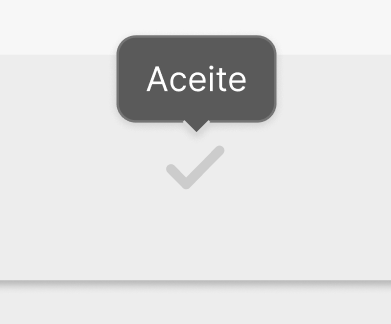
\includegraphics[width=0.2\textwidth]{res/prototype/estado-pedido-tooltip.png}
    \caption{\emph{Tooltip} sobre o estado de um pedido.}
    \label{estado-pedido-tooltip}
\end{figure}

\section{Componentes Implementados}

O primeiro passo no processo de implementação da interface foi a identificação de componentes e
respetiva implementação. Foram identificados como componentes \emph{widgets} comuns (botões, campos
de texto, \ldots) e outros elementos presentes em várias páginas / várias vezes na mesma página.
Note-se que \emph{widgets} simples foram implementados como componentes (em vez de serem usados
diretamente) para haver um maior controlo sobre o estilo que é aplicado aos mesmos, e para ser
possível suportar várias variantes dos mesmos. Segue-se uma breve lista dos vários componentes
desenvolvidos:

\subsection{Alerta}

Este componente estático apresenta uma informação importante ao utilizador. É utilizado, por
exemplo, para informar o utilizador na página ``Iniciar Sessão'' que as credenciais que submeteu
se encontram incorretas, ou nos componentes ``Aluno'' e ``Problema'' que um aluno é
trabalhador-estudante, como se vê na figura \ref{problem}.

\subsection{Barra de Navegação}

Este componente está presente no topo de todas as páginas implementadas, e permite ao utilizador
rapidamente navegar para outras páginas de interesse, bem como alterar o seu tema (claro ou escuro)
e terminar sessão. Este componente, como se vê abaixo, existe em três variantes, uma para antes de
se ter iniciado sessão, uma para alunos, e outra para o diretor de curso. A barra de navegação
subdivide-se em vários subcomponentes, que não serão mencionados neste relatório, visto que apenas
existem para dividir a barra de navegação em partes mais pequenas, dando origem a código mais
modular.

\begin{figure}[H]
    \centering
    
\includegraphics[width=\textwidth]{res/components/navbar-login.png}
    
\includegraphics[width=\textwidth]{res/components/navbar-student.png}
    
\includegraphics[width=\textwidth]{res/components/navbar-director.png}
    \caption{
        \onehalfspacing
        De cima para baixo, variantes de \emph{login}, de aluno, e do diretor de curso da barra de
        navegação.
    }
    \label{navbar}
\end{figure}

\subsection{Botão}

Este componente, presente em diversas páginas da aplicação, trata-se de um \emph{widget} no qual se
pode clicar para se realizar uma ação pré-determinada. Existem várias variantes de botão (ativo, de
cancelamento, e desativado), distinguíveis pela sua cor. Adicionalmente, botões desativados podem
ter uma \emph{tooltip} a explicar por que motivo não é possível interagir com eles. Abaixo,
apresentam-se os três tipos de botão implementados:

\begin{figure}[H]
    \centering
    
\includegraphics[width=\textwidth]{res/components/button.png}
    \caption{Da esquerda para a direita, variantes de cancelamento, desativada e ativa de botões.}
    \label{button}
\end{figure}

\subsection{Botão para Desfazer}

Este componente trata-se de um botão especial, utilizado para desfazer ações nas páginas
``Resolver Problemas'' e ``Gerir Turno''. Pode ser visto na figura abaixo:

\begin{figure}[H]
    \centering
    
\includegraphics[width=3cm]{res/components/undo-button.png}
    \caption{Botão para desfazer.}
    \label{undo-button}
\end{figure}

\subsection{Capacidade}

Este componente apresenta a utilização de um turno em função da sua capacidade, sendo utilizado na
página ``Gerir Turno'', no componente ``Turno'', e no diálogo de informação sobre um turno nas
páginas ``O Meu Horário'' e ``Horário Completo''. Opcionalmente, este componente pode passar a ser
representado a vermelho caso um turno exceda a sua capacidade, como pode ser visto na figura abaixo:

\begin{figure}[H]
    \centering
    
\includegraphics[width=4cm]{res/components/capacity.png}
    \caption{Capacidade de um turno sobrelotado.}
    \label{capacity}
\end{figure}

\subsection{Campo de texto}

Este componente, presente em várias páginas da aplicação, permite ao utilizador escrever texto a ser
consumido pelo programa. Existem três variantes deste componente, para entrada de texto, para
entrada de \emph{passwords}, e uma barra de pesquisa. Na figura abaixo, podem observar-se estas três
variantes do campo de texto:

\begin{figure}[H]
    \centering
    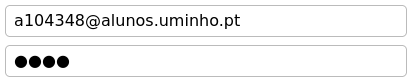
\includegraphics[width=8cm]{res/components/text-input-regular-password.png} \\
    
\includegraphics[width=8cm]{res/components/text-input-search.png}
    \caption{
        Campos de texto para entrada textual, entrada de \emph{passwords}, e barra de pesquisa.
    }
    \label{text-input}
\end{figure}

\subsection{\emph{Check box}}

Este componente permite ao utilizador definir o valor de um booleano. Destaca-se o seu uso no
componente ``Seletor de Turnos'', visível na figura \ref{shift-selector}.

\subsection{\emph{Dropdown}}

Presente apenas na página ``Gerir turno'', este componente permite ao utilizador escolher uma de
diversas opções, no caso, uma de diversas salas, como se pode ver abaixo:

\begin{figure}[H]
    \centering
    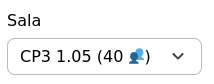
\includegraphics[width=4cm]{res/components/dropdown.png}
    \caption{\emph{Dropdown}.}
    \label{dropdown}
\end{figure}

\subsection{Estudante e Problema}

Estes dois componentes são bastante semelhantes, e permitem apresentar um estudante e um problema
(pedido de troca ou turno por atribuir), respetivamente. O componente ``Problema'' pode observar-se
abaixo:

\begin{figure}[H]
    \centering
    
\includegraphics[width=7cm]{res/components/problem.png}
    \caption{
        \onehalfspacing
        Problema de turno por atribuir. Caso apenas se apresentasse o aluno, a linha
        ``FCD T (por atribuir)'' não seria visível.
    }
    \label{problem}
\end{figure}

\subsection{Horário}

Este componente, utilizado em diversas páginas, permite apresentar um conjunto de turnos,
organizados temporalmente ao longo de uma semana, como se pode ver abaixo:

\begin{figure}[H]
    \centering
    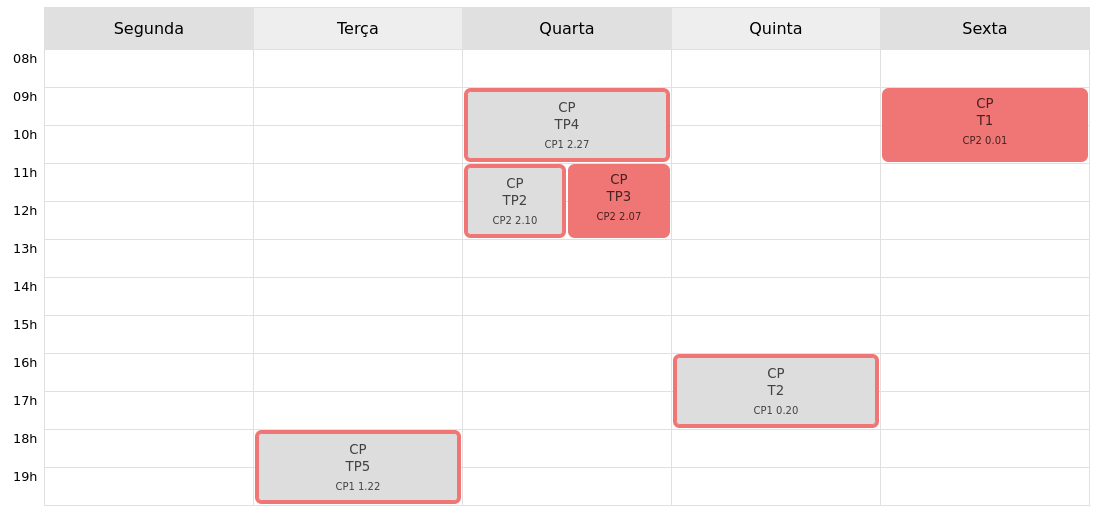
\includegraphics[width=0.45\textwidth]{res/components/schedule-1.png}
    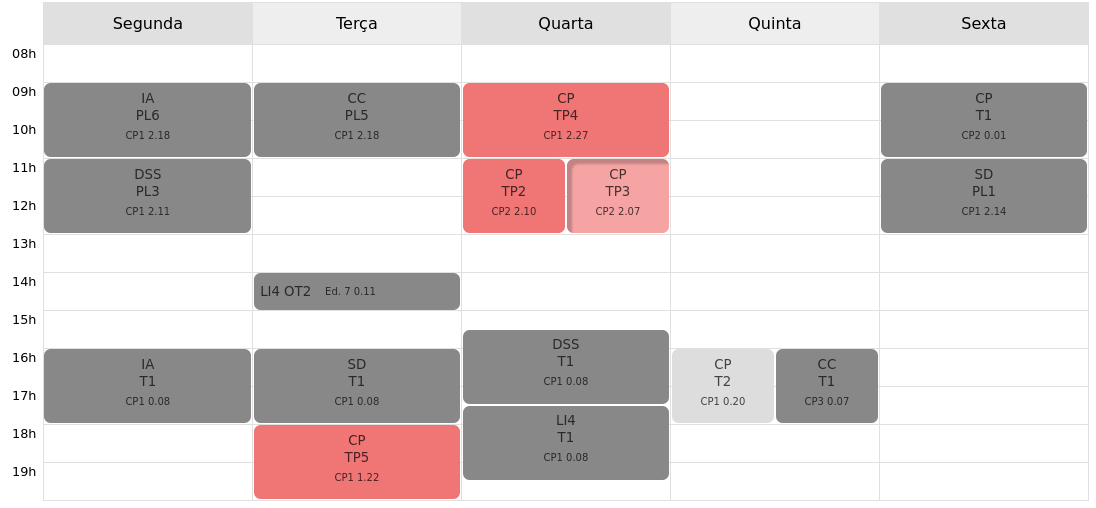
\includegraphics[width=0.45\textwidth]{res/components/schedule-2.png}
    \caption{Horários com diferentes tipos de turnos.}
    \label{schedule}
\end{figure}

\subsection{Ícone da Aplicação}

Este componente estático é usado na barra de navegação e na barra de janela do componente ``Popup''.
Pode ser visto na figura abaixo:

\begin{figure}[H]
    \centering
    
\includegraphics[width=4cm]{res/components/application-icon.png}
    \caption{Ícone da aplicação.}
    \label{application-icon}
\end{figure}

\subsection{Lista de Estudantes}

Este componente, utilizado na página ``Gerir Turno'', apresenta uma lista de estudantes, onde cada
estudante se encontra associado a um botão, que pode ser usado o para adicionar a / remover de um
turno. Este componente pode ser visto na figura abaixo:

\begin{figure}[H]
    \centering
    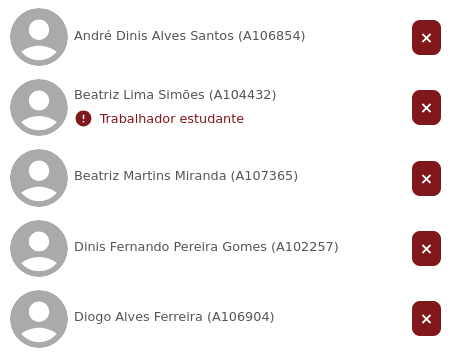
\includegraphics[width=10cm]{res/components/student-list.png}
    \caption{Lista para remoção de estudantes.}
    \label{student-list}
\end{figure}

\subsection{\emph{Popup}}

Este componente é um diálogo com uma borda de janela. Várias páginas utilizam \emph{popups}, mas
dois destes, para mostrar informação de um turno e para confirmar a troca entre dois turnos,
apresentados abaixo, foram transformados em componentes visto que estão presentes em mais do que uma
página, no caso, ``O meu Horário'' e ``Horário Completo''.

\begin{figure}[H]
    \centering
    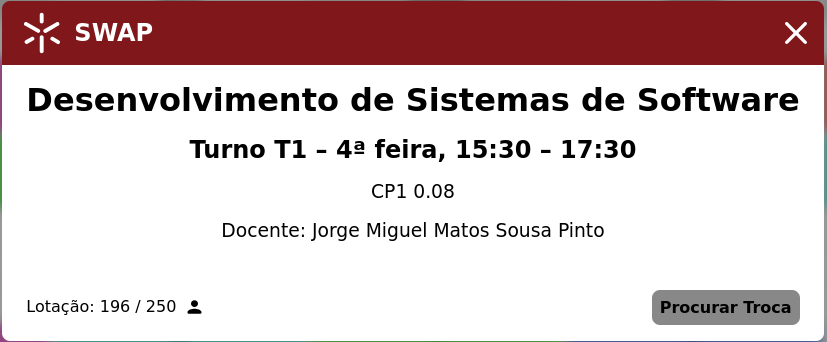
\includegraphics[height=4cm]{res/components/popup-1.png}
    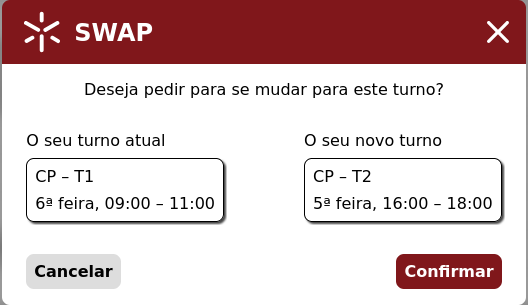
\includegraphics[height=4cm]{res/components/popup-2.png}
    \caption{Diálogos de informação de turno e para confirmação de troca de turnos.}
    \label{popup}
\end{figure}

\subsection{Seletor de turnos}

Este componente, presente nas páginas ``Horário Completo'' e ``Gerir Turnos'', permite ao utilizador
escolher que turnos deseja ver no horário.

\begin{figure}[H]
    \centering
    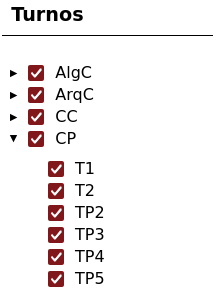
\includegraphics[width=4cm]{res/components/shift-selector.png}
    \caption{Seletor de turnos.}
    \label{shift-selector}
\end{figure}

\subsection{\emph{Toast}}

Este trata-se de um componente para apresentar um alerta ao utilizador, sem que este deixe de poder
utilizar a página. É normalmente utilizado para informar o utilizador de sucesso nas operações que
realizou: que um pedido de mudança de horário foi enviado nas páginas ``O Meu Horário'' e
``Horário Completo'', e que os horários foram publicados com sucesso, na página
``Resolver Problemas''. Abaixo, pode ver-se o exemplo de uma \emph{toast}:

\begin{figure}[H]
    \centering
    
\includegraphics[width=8cm]{res/components/toast.png}
    \caption{\emph{Toast}.}
    \label{toast}
\end{figure}

\subsection{Turno}

Este componente, utilizado no componente ``Horário'' (figura \ref{schedule}), permite apresentar um
turno. Existem várias variantes de turnos, necessárias para ser possível distinguir turnos com os
quais é possível interagir, turnos pertencentes ao horário do aluno, o turno do qual um aluno
requisita para sair, \emph{etc.}. É também possível escolher se se deseja que um turno apresente ou
não a sua capacidade.

\subsection{Botão com ícone}

Este componente trata-se de um \emph{widget} no qual se pode clicar para se realizar uma ação,
sendo utilizado no componente ``Notificação'', do diretor de curso (figura \ref{notification}).
Existem várias variantes para as ações de rejeitar, aprovar ou navegar para a página de resolução
de um pedido, distinguíveis pelo seu ícone. Abaixo podem ser vistos os três tipos do botão
implementados:

\begin{figure}[H]
    \centering
    
\includegraphics[width=4cm]{res/components/icon-button.png}
    \caption{Da esquerda para a direita, variantes de rejeição, aprovação e navegação dos botões.}
    \label{icon-button}
\end{figure}

\subsection{Notificação}

Este componente, utilizado no componente ``Lista de Notificações''
(figura \ref{notifications-list}), permite apresentar o conteúdo e estado
de uma notificação / pedido (trocas de turno, sala ou alertas).
Existem várias variantes (notificação de aluno, director de curso ou pedido), distinguíveis pelo
seu conteúdo. Adicionalmente, notificações do diretor de curso quando com o cursor em cima
apresentam três botões que permitem rejeitar, aprovar ou navegar para a página de resolução do
pedido de um aluno / professor. As variantes do diretor de curso e de um pedido podem-se
observar abaixo:


\begin{figure}[H]
    \centering
    
\includegraphics[width=\textwidth]{res/components/director-notification.png}
    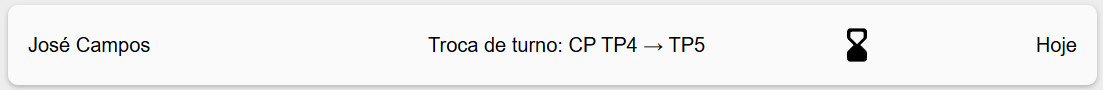
\includegraphics[width=\textwidth]{res/components/student-request.png}
    \caption{De cima para baixo, variantes notificação de diretor de curso e de pedido.}
    \label{notification}
\end{figure}

\subsection{Lista de Notificações}

Este componente, utilizado nas páginas de ``Histórico de Pedidos'' e ``Notificações'',
apresenta uma lista de notificações / pedidos, em que cada elemento é uma instância do componente
``Notificação''. Permite listar as notificações / pedidos de um utilizador, organizados
temporalmente e por estado do pedido, como se pode ver abaixo:


\begin{figure}[H]
    \centering
    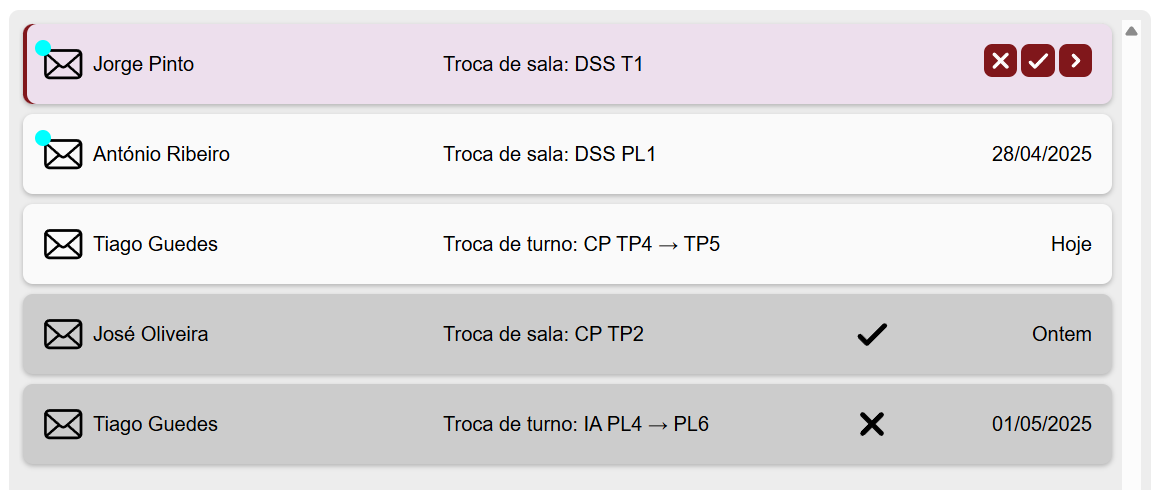
\includegraphics[width=\textwidth]{res/components/director-notifications-list.png}
    \caption{Lista de notificações, do diretor de curso.}
    \label{notifications-list}
\end{figure}

\section{Páginas Implementadas}

Para não repetir o mesmo conteúdo duas vezes neste relatório, as páginas implementadas são
apresentas na secção ``\nameref{user-manual}''.

\section{Tecnologias Utilizadas}

Para a realização deste projeto, foi necessário o uso de diversas tecnologias. Nesta secção,
procura-se apresentar as diversas tecnologias utilizadas, como estas foram utilizadas, e as
facilidades e dificuldades sentidas com cada uma.

\subsection{HTML e CSS}

Visto que a aplicação desenvolvida é uma aplicação Web, o uso de HTML e CSS é imperativo em quase
todas as \emph{frameworks}. De um modo geral, o desenvolvimento de componentes e páginas com recurso
a estas tecnologias foi fácil, especialmente devido à sua natureza declarativa. Outra facilidade do
uso destas tecnologias foram as flexboxes, que simplificaram a organização dos elementos nos
componentes e nas páginas.

No entanto, houve algumas dificuldades em garantir que o código desenvolvido funcionava em todos os
navegadores: como nem todos os navegadores suportavam todas as funcionalidades desejadas, foi
necessário testar a aplicação desenvolvida em Chromium (Blink), Firefox (Gecko) e Safari (WebKit).
Várias vezes, foi necessário adicionar regras de CSS com \emph{vendor prefixes}, ou até refazer
algumas funcionalidades devido a diferenças de funcionamento entre navegadores.

\subsection{TypeScript}

\hyphenation{Java-Script}

No projeto desenvolvido, foi utilizado TypeScript \cite{typescript}, linguagem que é transpilada
para JavaScript, mas que permite alguma verificação de tipos. O TypeScript foi uma grande ajuda para
garantir a correção do código da aplicação, e assegurar, em \emph{compile-time}, que a aplicação não
terá exceções em \emph{runtime} devido a erros de tipos. Ademais, o compilador não obriga que o
código seja tipado durante o processo de desenvolvimento, pelo que este pode continuar a ser
bastante veloz. Assim, apenas quando se acaba de escrever um módulo / componente / página, podem
adicionar-se anotações de tipo ao código para garantir a sua correção.

\subsection{Vue}

A \emph{framework} utilizada para o desenvolvimento da aplicação foi Vue.js \cite{vue}. Esta
\emph{framework}, devido à sua natureza declarativa e reativa, foi de muito fácil atualização:
alterar um objeto reativo conduzia à atualização automática das partes do componente / da página que
sofreram alterações. Por exemplo, ao contrário do Blazor \cite{blazor}, utilizado em Laboratórios de
Informática IV, não era necessário chamar uma função (\texttt{StateHasChanged}) sempre que era
necessário atualizar os conteúdos da DOM.

Apesar de poucas, foram sentidas algumas dificuldades no uso de Vue, especialmente quando era
necessário integrar funcionalidades não reativas (no caso, a resposta a um evento de mudança de uma
\emph{media query}) com a reatividade do Vue, tendo sido necessários \emph{hacks} para forçar a
atualização dos objetos reativos.

\subsection{Pinia}

A biblioteca Pinia \cite{pinia} foi utilizada para armazenamento do estado da aplicação, como as
credenciais do utilizador, o tema da aplicação (claro ou escuro) e os turnos escolhidos nas páginas
``Horário Completo'' e ``Gerir Turnos'', para que esta informação não desapareça quando se navega
entre diferentes páginas da aplicação. Adicionalmente, o \emph{plugin}
\texttt{pinia-plugin- persistedstate} \cite{pinia-persistent} foi utilizado para persistir algum
estado no \texttt{localStorage} do navegador, para este ser mantido mesmo após o navegador ser
fechado. Por exemplo, as credenciais do utilizador são armazenadas no \texttt{localStorage} quando
este escolhe que deseja que a aplicação se ``lembre de si''.

O Pinia, devido à sua integração com Vue, foi das ferramentas de mais fácil utilização, visto que os
objetos armazenados nos \emph{stores} do Pinia podiam ser utilizados como qualquer outro objeto
reativo do Vue.

\subsection{JSON Server}

É necessário que a aplicação desenvolvida tenha dados que possa apresentar. Na UC de Interface
Pessoa-Máquina, não é pedido que se implemente um \emph{backend} completo para a aplicação, pelo que
se utilizou \texttt{json-server} \cite{json-server}, um programa que cria uma API REST a partir dos
dados num ficheiro JSON.

A utilização desta tecnologia foi complicada, não devido a complexidade da tecnologia em si, mas sim
devido ao trabalho necessário para organizar os dados da API num formato adequado para apresentação.
Devido às capacidades muito limitadas de interrogação do \texttt{json-server}, várias interrogações
tiveram de ser implementadas imperativamente em JavaScript, ao contrário de declarativamente numa
linguagem especializada, como se teria feito caso se tivesse utilizado uma base de dados. O uso de
uma base de dados seria, por este motivo, uma grande melhoria ao projeto.

\subsection{Outras tecnologias}

O \texttt{npm} \cite{npm} é o gestor de pacotes do NodeJS, que permite, no ficheiro
\texttt{pacakage.json}, definir as dependências do projeto desenvolvido. Além disso, também é
possível definir \emph{scripts} como \texttt{npm run dev}, para abrir a aplicação com ferramentas de
desenvolvimento, e \texttt{npm run preview}, para pré-visualização da aplicação final. Para melhorar
a experiência de desenvolvimento, estes dois \emph{scripts} foram modificados para, além de
executarem o servidor HTTP da aplicação, também executarem o JSON Server. Também foram adicionados
\emph{scripts} para, com recurso às ferramentas ESLint \cite{eslint} e Prettier \cite{prettier},
automaticamente fazer uma análise estática e formatação do código, respetivamente. Estes
\emph{scripts} são usados na \emph{pipeline} de CI (\emph{Continuous Integration}) do repositório do
projeto (GitHub Actions), obrigando a que todos os \emph{pull requests} tenham código correto e bem
formatado.

A principal dificuldade do uso do \texttt{npm} foi garantir que os \emph{scripts} criados
funcionavam em diferentes sistemas operativos, visto que alguns comandos utilizados apenas estavam
disponíveis, por exemplo, em Linux.

\section{Manual de Utilização}
\label{user-manual}

\section{Reflexão sobre a Aplicação}

\section{Conclusão}

\begingroup
\section{Bibliografia}
\renewcommand{\section}[2]{}

\begin{thebibliography}{9}
    \bibitem{vue}
        ``The Progressive JavaScript Framework''. Figma. Accessed: Apr. 30, 2025. [Online.]
        Available: \url{https://vuejs.org/}
    \bibitem{figma}
        ``Figma: Collaborative Interface Design Tool''. Figma. Accessed: Mar. 13, 2025. [Online.]
        Available: \url{https://www.figma.com/}
    \bibitem{typescript}
        ``TypeScript''. TypeScript. Accessed: Apr. 30, 2025. [Online.] Available:
        \url{https://www.typescriptlang.org/}
    \bibitem{blazor}
        `` Launch your idea to the web fast with Blazor''. Blazor. Accessed: Apr. 30, 2025.
        [Online.] Available: \url{https://dotnet.microsoft.com/en-us/apps/aspnet/web-apps/blazor}
    \bibitem{pinia}
        ``Pinia: The intuitive store for Vue.js''. Pinia. Accessed: Apr. 30, 2025. [Online.]
        Available: \url{https://pinia.vuejs.org/}
    \bibitem{pinia-persistent}
        ``Pinia Plugin Persistedstate: Configurable persistence of Pinia stores''.
        Pinia Plugin Persistedstate. Accessed: Apr. 30, 2025. [Online.] Available:
        \url{https://prazdevs.github.io/pinia-plugin-persistedstate/}
    \bibitem{json-server}
        ``json-server''. GitHub. Accessed: Apr. 24, 2025. [Online.] Available:
        \url{https://github.com/typicode/json-server}
    \bibitem{npm}
        ``NPM''. NPM. Accessed: Apr. 24, 2025. [Online.] Available: \url{https://www.npmjs.com/}
    \bibitem{eslint}
        ``ESLint''. ESLint. Apr. 24, 2025. [Online.] \url{https://eslint.org/}
    \bibitem{prettier}
        ``Prettier''. Prettier. Apr. 24, 2025. [Online.] \url{https://prettier.io/}
\end{thebibliography}
\endgroup

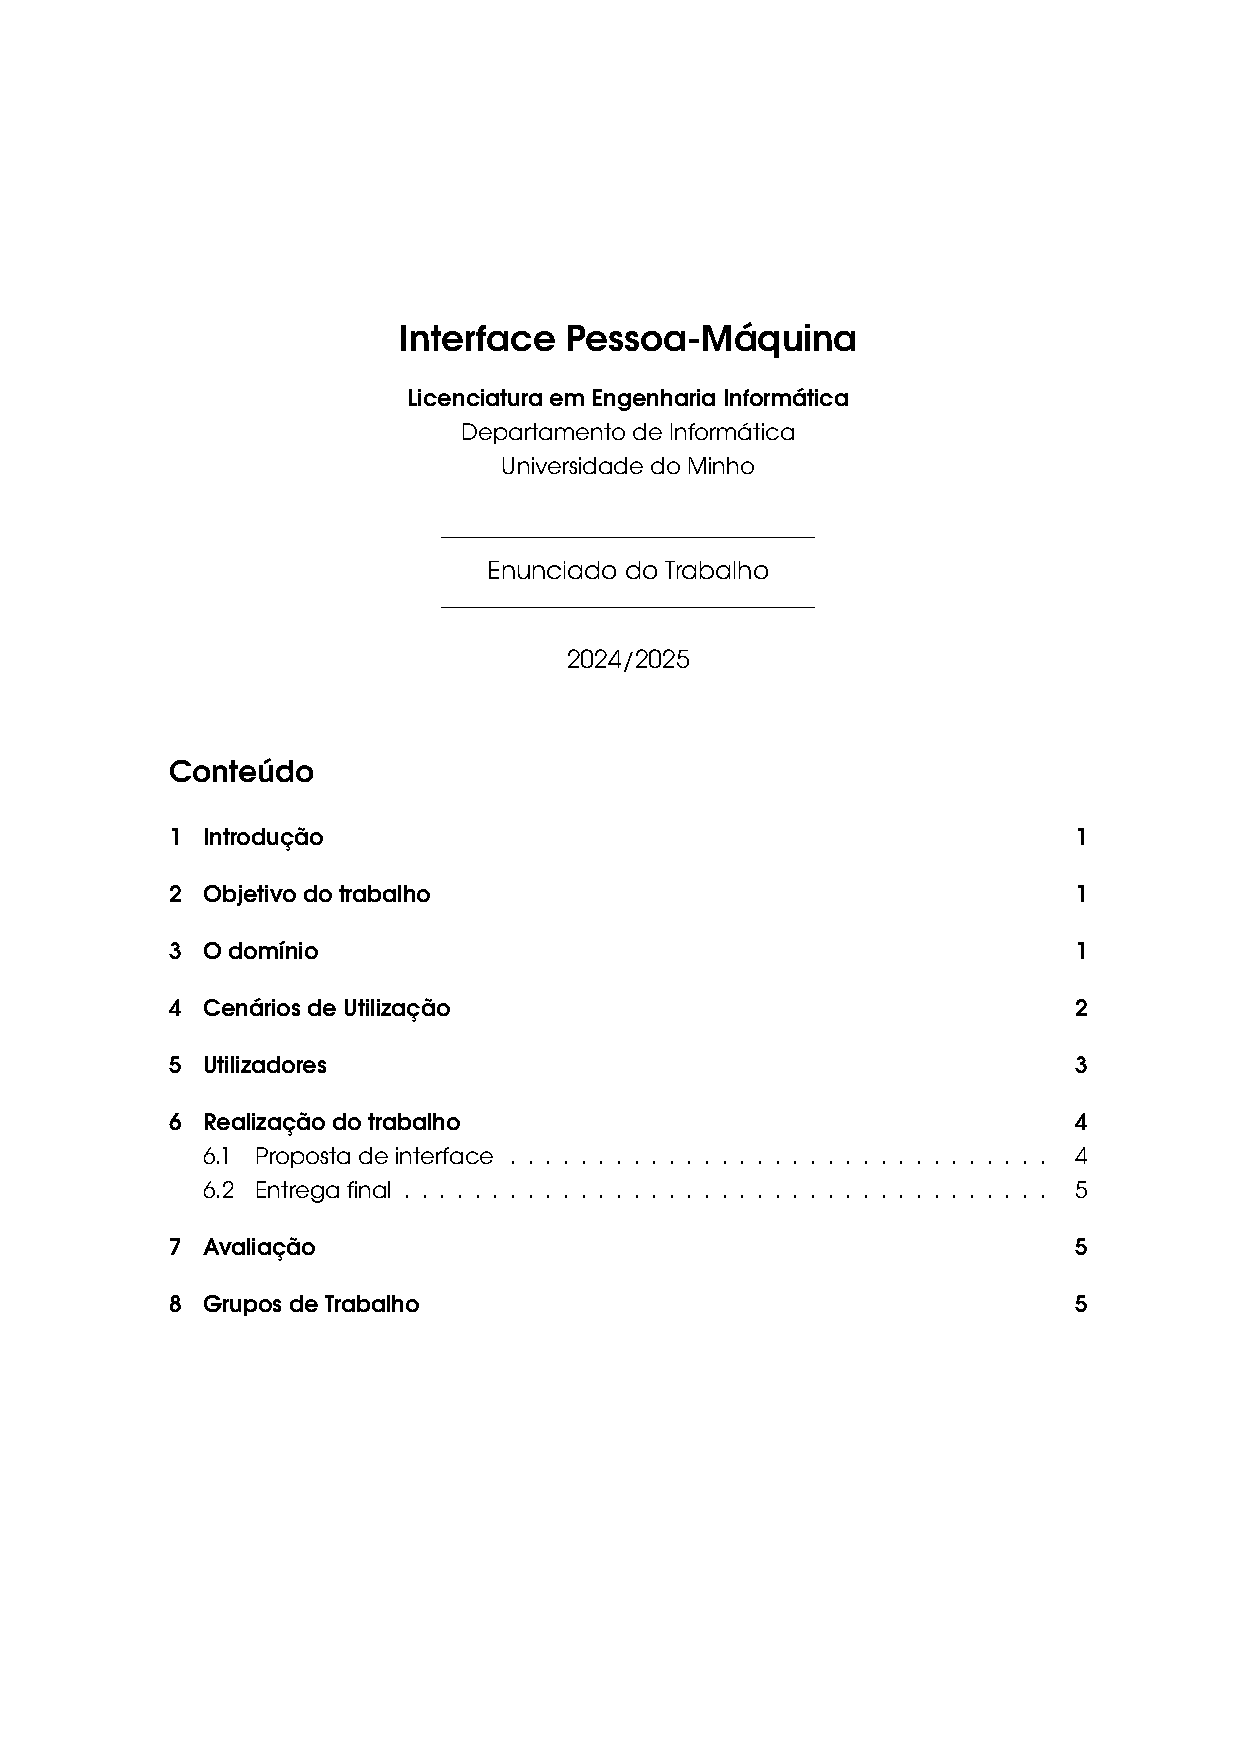
\includepdf[pages=1,pagecommand=\section{Anexo -- Enunciado do Trabalho}\thispagestyle{empty}]
    {../Assignment.pdf}
\includepdf[pages=2-]{../Assignment.pdf}

\end{document}
